\chapter{Fundamentação teórica e metodologia}

\section{\dBG}

% - Detailed explanation of \dBG of a set of DNA sequences
%   - reverse complements
% - How it is going to be used
% - Operations
%   - Insert node
%   - Insert edge
%   - Query node
%   - Query edge / star 
% - Space-efficient representations - that's what we propose

The \dBG is a directed graph for which each node represents a sequence of symbols, and each edge between two nodes represents
the overlap between the two sequences. That is, given two nodes on the graph, they each represent a distinct sequence of symbols
$S_1$ and $S_2$, and there is an edge between them if and only if the tail of $S_1$ is the head of $S_2$.

Within the context of genome sequencing, \dB graphs are used in the assembly process by storing the distinct \kmer 's identified
in the read sequences. In the ideal case (when each \kmer is present only once in the original sequence, and there are no
sequencing errors), the complete traversal of this graph would produce the original sequence. In practice, such a straightforward
approach is not feasible, but the \dBG can still be used to produce longer sequences, called \emph{contigs}, which can then be processed
to assemble the original genome. Figure~\ref{fig:dbgexample} presents an example of the \dBG within this context.

\begin{figure}[htbp]
	\begin{center}
    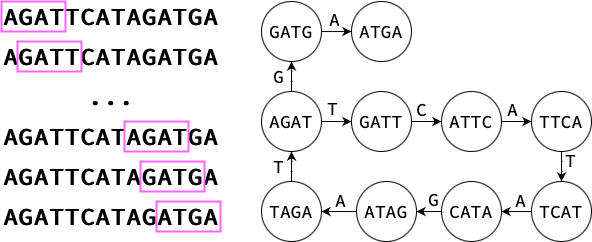
\includegraphics[width=0.8\textwidth]{figures/dbg-example}
	\end{center}
	\caption{Example of a \dBG. $k=4$}\label{fig:dbgexample}
\end{figure}

In a strict definition of a \dBG, the graph must support insertion operations for both nodes and edges. It has long been understood,
however, that storing both node and edge information is redundant, and having only one of the two is sufficient to represent the graph.
In a similar way, the \dBG must allow for the query operation of nodes and edges. In practice, however, only one of these is needed.

\subsection{Reverse Complements}

One individuality of the genome sequencing context is the presence of \emph{reverse complements}. When generating sequencing reads,
a sequence of DNA can be read both in its forward form, or in its reverse complement. That is, the read is generated not from the
original sequence $S$, but its complement $\overline{S}$, generated by swapping each base with its Watson-Crick complement
($\A \leftrightarrow \T$, $\C \leftrightarrow \G$). As in \cite{Conway2011}, this will be treated by processing all reads in both
directions, without, however, merging nodes representing reverse complements. As noted by Conway \& Bromage: ``This makes the graph
symmetric; a forward traversal corresponds to a backwards traversal on the reverse complement path, and vice versa.``\cite{Conway2011}.

\subsection{Representing a \dBG}

Due to its nature, a \dBG can be represented by its set of nodes or edges independently, as one can be derived from the other.
\asq{Citation needed} As such, a structure that can answer queries about the presence of a given node on the graph is enough to
represent the graph. In this regard, Conway \& Bromage showed that a lower bound on the number of bits required to \emph{exactly}
represent a \dBG exists, and is $\Omega(n \log n)$, for $n$ being the number of distinct \kmer's present in the graph, and $4^k > n$
\cite{Conway2011}.

In order to further improve space-efficiency, new forms of representation were created that XXX exactness for a probabilistic approach
such as \emph{Navigational Data Structures} (NDS), which have some probability of giving an erroneous answer to a membership query, 
but can be used to navigate the graph. This definition is useful due to the fact that a \dBG is not queried for the membership of randomly
selected nodes, but rather only the neighborhood of a known member node is queried\cite{Chikhi2014}. In sections \ref{sec:debruijncountmin}
and \ref{sec:debruijnhashtable} we will introduce two new NDS's.

\section{\cm}
\label{sec:countmin}

The \cm sketch, first introduced in \cite{Cormode2005}, is a sub-linear data structure intended to allow for event frequency mapping.
In this way, it must allow for the query of the frequency of a given event, as well as the update of that frequency, through the
\emph{query} and \emph{update} operations. The sketch is composed of a $W$-wide, $D$-deep matrix of counters. With each row in this
matrix is associated a hash function that map the possible events to the $W$ positions in that row, such that all $D$ hash functions
must be pair-wise independent.

Updating the frequency of a given event is done by passing it through the hash functions for each row, and then updating the counter in
the resulting position accordingly.

Querying the structure consists of, similarly, retrieving the value of the counter associated with the key in each row, and then returning
the minimum value among them.

Figure \ref{fig:countminexample} presents a visualization of the \cm sketch.


\begin{figure}[htbp]
	\begin{center}
    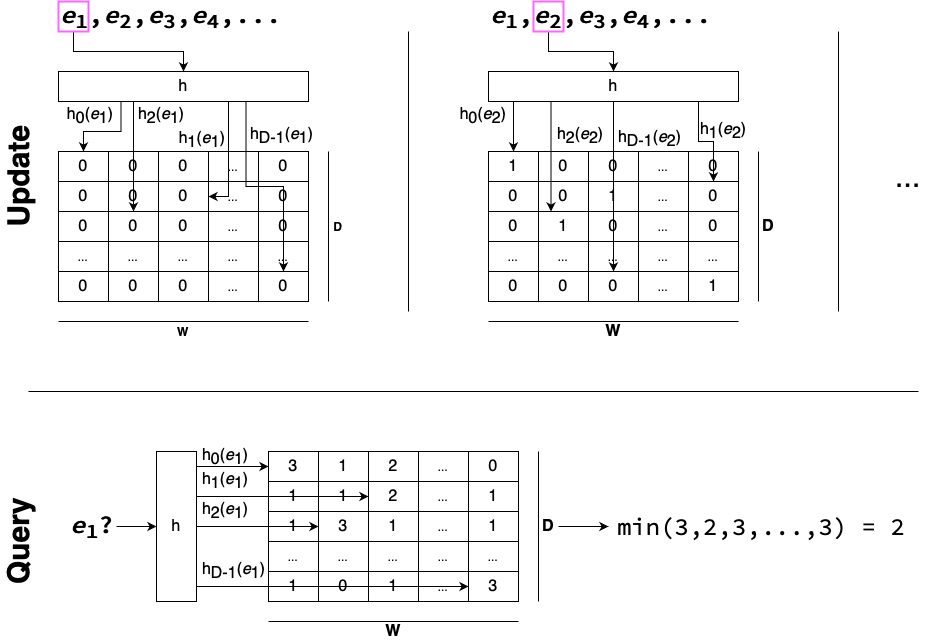
\includegraphics[width=0.8\textwidth]{figures/cm-example}
	\end{center}
	\caption{Example of a \cm sketch being used to count \kmer's. $k=4$}\label{fig:countminexample}
\end{figure}

\subsection{As a representation for a \dBG}

\asq{Vale colocar isso aqui, ou é mais interessante deixar apenas para falar disso no capítulo anterior (State of the Art), quando falando
sobre o \emph{FastEtch}?}

A \cm sketch can implement the membership query operation by querying the count for a given \kmer and comparing it to a presence threshold:
if the count surpasses this threshold, the \kmer is considered to be present in the \dBG, and if the count is inferior to the threshold the
\kmer is considerent absent from the graph.

\section{\dBCM}
\label{sec:debruijncountmin}

% - Representation (what goes in each cell)
% - Operations:
%   - addOutEdge
%   - query 
% - Analysis space/time (may be done within previous sections)

In order to this work we introduce a modified version of the \cm sketch, which we call the \dBCM, that allows the sketch to be queried not only
for \kmer counts, but also for the edges from the \dBG associated with that \kmer. In this way we expect to improve navigability of the
graph through the sketch allowing for the construction of the \dBG online.

In order to store the additional information, we expand the \cm sketch such that each cell in the matrix stores not only the counter,
but also a set of out edges. The structure, then, provides an interface to increment the counters associated with a given key by one,
and an interface to add an out edge to the sets associated with a given key. The increment operation is performed in the same way as in
a regular \cm sketch, and the algorithm for the add edge operation can be seen in Algorithm \ref{alg:addOutEdge}.

Furthermore, the \dBCM must accomodate this new information in its query operation. In order to do this, the sketch returns not only
the minimum value of the counters, but also the intersection of the sets of out edges. The algorithm for the updated query operation is
described in Algorithm \ref{alg:query}.

\begin{algorithm}[htbp]
    \caption{$\mathit{addOutEdge}(\text{k-mer}, \mathit{outEdge})$}\label{alg:addOutEdge}
    \KwData{$\mathit{outEdge} \in \{\A, \C, \G, \T\}$}
    \For{$i = 1, \ldots, D$}{
      $\mathit{CountMin}[i][h_i(\text{k-mer})].\mathit{outEdges} \gets \mathit{CountMin}[i][h_i(\text{k-mer})].\mathit{outEdges} \cup \mathit{outEdge}$\;
    }
\end{algorithm}

From a practical perspectie, due to a node only ever having 4 possible out edges (corresponding to the 4 bases $\{\A, \C, \G, \T\}$),
the set of out edges can be represented by a bit vector indicating whether each of these possible edges is present. An edge is added
by setting the corresponding bit, and the intersection is obtained by performing the bitwise AND operation. This allows both set of
out edges and the counter to be stored together in a single integer.

\begin{algorithm}
    \caption{$\mathit{query}(\text{k-mer})$}\label{alg:query}
    $\mathit{count} \gets \mathit{inf}$\;
    $\mathit{outEdges} \gets \{\A, \C, \G, \T\}$\;
    \For{$i = 1, \ldots, D$}{
      $\mathit{count} \gets \min(\mathit{count}, \mathit{CountMin}[i][h_i(\text{k-mer})].\mathit{count})$\;
      $\mathit{outEdges} \gets \mathit{outEdges} \cap \mathit{CountMin}[i][h_i(\text{k-mer})].\mathit{outEdges}$\;
    }
    \Return{$(\mathit{count}, \mathit{outEdges})$}
\end{algorithm}

\subsection{As a representation of a \dBG}

\section{Hashtable}
\label{sec:debruijnhashtable}
% - Structure
%   - fingerprint
%   - Outedges
% - Hash function 
% - Collision resolution
% - Operations 
%   - Add node/edge
%   - Query node/edge/star 
% - Analysis 

We also propose a new hashtable-based representation for the \dBG that is made more efficient by not storing the \kmer. Instead,
a fingerprint generated from the \kmer is stored, along with the set of out edges as described in Section \ref{sec:debruijncountmin}.
When a \kmer is inserted into the hashtable, or queried from it, a hash value and a fingerprint are calculated in parallel.
In case of an insertion, the fingerprint is written at the desired position and, on a query, the fingerprints are compared. Collisions
are resolved by linear probing, such that if a key tries to insert in a position that is already occupied by a fingerprint that doesn't 
match its own, the \kmer is inserted in the next free position, unless its fingerprint is found before a free position is. During the
query this process is repeated until the desired fingerprint is found, or a free position is reached (in which case the \kmer is
considered to be absent from the structure).

This operation allows for the insertion of a node by adding the \kmer to the hashtable, and the insertion of an edge by updating the
edge set associated with the given \kmer. When queried, the structure returns the edge set associated with the given \kmer, provided
the \kmer has been added to the structure.

\section{A pipeline using the \dBCM and the \dBHT}

% Sequence ---(insert)---> Mod \cm ---(traverse)---> Hashtable 

Beyond the two isolated datastructures to represent the \dBG, we also propose a way to use both of them in tandem in order to obtain
the benefits of both. In this pipeline, the sequencing reads are processed and inserted into the \dBCM as they are made available,
such that the \dBG can be constructed online. Once the reads are all processed in this manner, and a navigatable version of the graph 
has been constructed, it can be traversed, with all of its nodes being, then, inserted in a \dBHT. In this way, a \dBCM is effectively
compressed into a \dBHT.

\section{Experiments}

\subsection{Metrics}

Through the experiments described further in this section, we evaluate different metrics for the \dBCM and the \dBHT. This is due to
the fact that both these structures have different goals and are used in different contexts.

As both of these structures are probabilistic in nature, however, there are certain metrics that are used in the evaluation of both.
One such metric is the \emph{false positive rate}. In this work, we define this rate based on the \kmer's that are visited during a 
traversal of the graph. Let $S$ be a genetic sequence that contains the set of \kmer's $K$, and let $G$ be the graph, represented
either by a \dBCM or a \dBHT, constructed from the sequencing reads of $S$. Further, let $Q$ be the set of \kmer's that were queried
from $G$ during its traversal, and $P={k | k \in Q \wedge k \in G}$ be the set of queried \kmer's that were in $G$. As such, we can
define the set of false positives as $F_P=P \setminus K$ (i.e.: the set of \kmer's that were queried and found to be in $G$ but are not
actually in the original sequence $S$). Finally, the false positive rate is defined as $fp=\frac{|F_P|}{|Q|}$ (i.e.: the ratio of false
positives to the total number of \kmer's that were queried during traversal of $G$).

\asq{Realmente vale a pena tentar fazer isso ainda? Estamos na reta final do projeto já, e isso iria requerer a definição do que é uma
mudança significativa nos resultados que justifique a mudança na estrutura}

Further, as we posit that being able to answer neighborhood queries will improve navigability of the graph by reducing the number of
membership queries made and, thus, the number of false positives, we perform two traversals of the \dBG, the first without using the
out edges information (i.e.: for every node that is in the graph, we query all possible neighboring nodes), and the second with that
information (i.e.: only recorded out edges are used to expand the frontier). We, then, compare the different metrics for the two
traversals.

\subsubsection{\dBCM}

The \dBCM was developed to be used directly with the sequencing reads without any pre-processing. It's goal is to build a reliable
navigatable version of the \dBG as the reads are made available. In this context, not only do we expect a certain amount of false
positives will appear, but as we must probabilistically filter the set of \kmer's from the reads to remove all the spurious ones, we
also expect the occurence of \emph{false negatives}, which are defined as \kmer's from the original sequence $S$ that are not present
in the graph $G$. I.e.: $F_N=K \setminus P$. As such, the \emph{false negative rate} can be defined as the ratio of false negatives
to the total number of \kmer's in the original sequence $S$, or $fn=\frac{|F_N|}{|K|}$.

\subsubsection{\dBHT}

\subsection{\emph{E.~Coli}}

The \emph{E.~Coli} genome is an established benchmark for new assemblers to compare against.

We used the reference genome for the \emph{E.~Coli} bacterium available in \url{http://ftp.ensemblgenomes.org/pub/bacteria/release-52/fasta/bacteria_0_collection/escherichia_coli_str_k_12_substr_mg1655_gca_000005845/dna/}

Three different experiments were performed. In the first we generated simulated perfect reads from the genome by taking substrings of 
the original sequence at random. We then used the \emph{ART Illumina} toolkit \asq{Citation needed} to simulate realistic reads from this
genome, including read errors and reverse complements. Finally, a dataset of real-world reads was downloaded from SRA \asq{Citation Needed}
and used.

\subsubsection{Synthetic reads without errors}

Given the reference genome $S$, the length of each read, $L$, and the desired coverage $C$, the synthetic reads were generated by picking
$\frac{|S| \times C}{L}$ substrings of $S$ at random. This is presented in algorithmic form in Algorithm \ref{alg:generate-reads}.

\begin{algorithm}
  \caption{Generate Reads}\label{alg:generate-reads}
  \KwData{$S$, the reference genome, $L$ the read length, $C$ the coverage}
  $\mathit{\#reads} \gets \frac{|S| \times C}{L}$\;
  $reads \gets \emptyset$\;
  \For{$i \gets 1, \ldots, \mathit{\#reads}$}{
    $j \gets \mathit{random}(0, |S| - L)$\;
    $\mathit{reads.add}(S[j: j+L])$\;
  }
  \Return{$reads$}
\end{algorithm}

\subsubsection{Synthetic reads with errors}

In order to simulate the reads as they would be produced by the sequencing process, we used the ART Illumina toolkit to generate
synthetic reads from the \emph{E.~Coli} genome. The reads were generated using the following parameters:

\begin{enumerate}
\item \textbf{Sequencing System}: Illumina MiSeq v3
\item \textbf{Read length}: \textit{250bp}
\item \textbf{Coverage}: \textit{80x}
\end{enumerate}